\documentclass[12pt]{article}
\usepackage[paper=letterpaper,margin=2cm]{geometry}
\usepackage{amsmath}
\usepackage{amssymb}
\usepackage{amsfonts}
\usepackage{newtxtext, newtxmath}
\usepackage{enumitem}
\usepackage{titling}
\usepackage{svg}
\usepackage{xcolor}
\usepackage{listings}
\usepackage{float}
\usepackage{nicefrac}
\usepackage{multirow}
\usepackage{fancyhdr}
\usepackage[most]{tcolorbox}
\usepackage[colorlinks=true]{hyperref}

\setlength{\droptitle}{-6em}

\definecolor{codegreen}{rgb}{0,0.6,0}
\definecolor{codegray}{rgb}{0.5,0.5,0.5}
\definecolor{codepurple}{rgb}{0.58,0,0.82}
\definecolor{backcolour}{rgb}{0.95,0.95,0.92}
\definecolor{bg}{rgb}{1,0.96,0.9}

\lstdefinestyle{mystyle}{
  commentstyle=\color{codegreen},
  keywordstyle=\color{magenta},
  numberstyle=\tiny\color{codegray},
  stringstyle=\color{codepurple},
  basicstyle=\ttfamily\footnotesize,
  breakatwhitespace=false,
  breaklines=true,
  captionpos=b,
  keepspaces=true,
  numbers=left,
  numbersep=5pt,
  showspaces=false,
  showstringspaces=false,
  showtabs=false,
  tabsize=2
}

% \tcbset{enlarge left by=-0.8cm,left=1.2cm,enlarge right by=-2cm,right=0.8cm}

\lstset{
  style=mystyle,
  inputencoding=utf8,
  extendedchars=true,
}

\newcommand{\question}[1]{\begin{tcolorbox}[enhanced jigsaw,colback=bg,boxrule=0pt,arc=1pt,halign=center] #1 \end{tcolorbox}}

\pagestyle{fancy}
\lhead{ML Exercises - 2022/23}
\rhead{Problem Set 4}

\begin{document}

The $k$NN, or $k$-nearest neighbors algorithm, is a simple supervised learning algorithm,
which works under the assumption that samples with similar features are more likely to
share the same label. The algorithm is very straight-forward, although differing
between trying to predict categoric and numeric labels: using a given distance
metric (such as Euclidean, Manhattan, etc.), the algorithm finds the $k$ closest samples to
the sample we want to classify, and assigns the label that:

\begin{enumerate}
  \item is most common (i.e. the mode) among the $k$ neighbors, in the case of categoric labels;
  \item is the average of the labels of the $k$ neighbors, in the case of numeric labels.
\end{enumerate}

\begin{enumerate}[leftmargin=\labelsep]
  \question {
  \item Considering the following data set:

        \begin{table}[H]
          \centering
          \begin{tabular}{c|cc|cc}
                  & $y_1$ & $y_2$ & $z_1$ & $z_2$ \\ \hline
            $x_1$ & 1     & 1     & A     & 1.4   \\
            $x_2$ & 2     & 1     & B     & 0.5   \\
            $x_3$ & 2     & 3     & B     & 2     \\
            $x_4$ & 3     & 3     & B     & 2.2   \\
            $x_5$ & 2     & 2     & A     & 0.7   \\
            $x_6$ & 1     & 2     & A     & 1.2
          \end{tabular}
        \end{table}

        Assuming $k$NN, with $k=3$ applied within a leave-one-out schema:

        \begin{enumerate}
          \item Considering an $z_1$ categoric output variable and the Euclidean distance,
                provide the prediction for $x_1$.
          \item Considering an $z_2$ numeric output variable and the cosine similarities,
                provide the mean regression estimate for $x_1$.
          \item Considering a weighted-distance $k$NN, with Manhattan distance, identify both the
                \textbf{weighted-mode} estimate of $x_1$ for a $z_1$ outcome and the
                \textbf{weighted-mean} estimate of $x_1$ for a $z_2$ outcome.
        \end{enumerate}
        }

        Here, working with a leave-one-out schema means that, for each sample, we
        can pick its $k$ neighbors from the pool of all the other samples, excluding
        itself (which, in theory, is always its closest neighbor, with null distance).

        \begin{enumerate}
          \item {
                The Euclidean distance is defined as the square root of the sum of the squared
                differences between the features of the two samples:

                \begin{equation*}
                  d(x_i, x_j) = \sqrt{\sum_{l=1}^p (x_{i}^{(l)} - x_{j}^{(l)})^2}
                \end{equation*}

                Since we're working with a leave-one-out schema, and trying to estimate
                the $z_1$ label for $x_1$, we can pick the $k$ neighbors from all
                samples except $x_1$. Below are illustrated the Euclidean distances
                between those samples and $x_1$, with the $k$ closest neighbors highlighted
                in teal:

                \begin{align*}
                  d(x_1, x_2) = \sqrt{(1 - 2)^2 + (1 - 1)^2} = \textcolor{teal}{1}
                \end{align*}
                \begin{align*}
                  d(x_1, x_3) = \sqrt{5}  , \quad
                  d(x_1, x_4) = 2 \sqrt{2}, \quad
                  d(x_1, x_5) = \textcolor{teal}{\sqrt{2}}  , \quad
                  d(x_1, x_6) = \textcolor{teal}{1}
                \end{align*}

                Knowing the $k$ closest neighbors, we can now estimate the $z_1$ label
                for $x_1$, by picking the most common label among them. In this case,
                the estimated label will be $\mathbf{mode} (B, A, A) = A$.
                }
          \item {
                Here, instead of the usual Euclidean/Manhattan distance, we're using the
                cosine similarities, which are defined as the cosine of the angle between
                the two vectors of features. As we know since high school, the cosine of
                the angle between two vectors is equal to the dot product of the two
                vectors divided by the product of their norms:

                \begin{equation*}
                  \cos(\vec{a}, \vec{b}) = \frac{\vec{a} \cdot \vec{b}}{\|\vec{a}\| \|\vec{b}\|}
                \end{equation*}

                Here, each sample is essentially a vector of features, hence the usage
                of this distance metric. The higher the cosine similarity, the closer
                the two vectors are, and vice versa: the cosine is equal to 1 when the
                two vectors are identical, and 0 when they are orthogonal.

                Let's now compute the cosine similarities between $x_1$ and the other
                samples, picking the $k$ closest neighbors (once again, in teal):

                \begin{align*}
                  \cos(x_1, x_2) = \frac{1 \cdot 2 + 1 \cdot 1}{\sqrt{2} \sqrt{5}} = \frac{3}{\sqrt{10}} = 0.94868, \quad
                  \cos(x_1, x_3) = \frac{1 \cdot 2 + 1 \cdot 3}{\sqrt{2} \sqrt{13}} = \frac{5}{\sqrt{26}} = \textcolor{teal}{0.98058}
                \end{align*}

                \begin{align*}
                  \cos(x_1, x_4) = \frac{1 \cdot 3 + 1 \cdot 3}{\sqrt{2} \sqrt{18}} = \frac{6}{\sqrt{36}} = \textcolor{teal}{1}, \quad
                  \cos(x_1, x_5) = \frac{1 \cdot 2 + 1 \cdot 2}{\sqrt{2} \sqrt{8}} = \frac{4}{\sqrt{16}} = \textcolor{teal}{1}
                \end{align*}

                \begin{align*}
                  \cos(x_1, x_6) = \frac{1 \cdot 1 + 1 \cdot 2}{\sqrt{2} \sqrt{5}} = \frac{3}{\sqrt{10}} = 0.94868
                \end{align*}

                Note, as mentioned above, that the closest neighbors here are the ones
                with a higher cosine similarity: $x_3$, $x_4$, and $x_5$. Since we're
                working with numeric labels for $z_2$, we can now estimate the mean
                regression estimate for $x_1$ by averaging the values of $z_2$ for those
                samples. In this case, the estimated value will be $\mathbf{mean} (2, 2.2, 0.7) = 1.6(3)$.
                }
          \item {
                Note that, here, we're working with a weighted-distance $k$NN, which means
                that we're assigning different weights to each sample based on its distance
                from the sample we're trying to estimate - a closer neighbor will have a
                bigger impact on the final estimate than a further neighbor. Note, also,
                that we're now working with the Manhattan distance, which is defined as
                the sum of the absolute differences between the features of the two samples:

                \begin{equation*}
                  d(x_i, x_j) = \sum_{l=1}^p |x_{i}^{(l)} - x_{j}^{(l)}|
                \end{equation*}

                Let's now compute the Manhattan distances between $x_1$ and the other
                samples, picking the $k$ closest neighbors (once again, in teal):

                \begin{align*}
                  d(x_1, x_2) = |1 - 2| + |1 - 1| = \textcolor{teal}{1}
                \end{align*}

                \begin{align*}
                  d(x_1, x_3) = 3, \quad
                  d(x_1, x_4) = 4, \quad
                  d(x_1, x_5) = \textcolor{teal}{2}, \quad
                  d(x_1, x_6) = \textcolor{teal}{1}
                \end{align*}

                Now, the fun part begins: we have to correctly weigh each neighbor's label
                to estimate the label for $x_1$. We can do this by assigning a weight to
                each neighbor, based on its distance from $x_1$. The most common way to
                do this is by using the inverse of the distance. Regarding the weighted
                mode estimate of $x_1$ for $z_1$:

                \begin{align*}
                  \hat{z}_1 = \mathbf{weighted\_mode} (\nicefrac{1}{1} B, (\nicefrac{1}{1} + \nicefrac{1}{2}) A) = A
                \end{align*}

                The mean, of course, will take into account for the denominator the
                weights of each neighbor, instead of the amount of neighbors:

                \begin{align*}
                  \hat{z}_2 = \mathbf{weighted\_mean} = \frac{\nicefrac{1}{1} \cdot 0.5 + \nicefrac{1}{2} \cdot 0.7 + \nicefrac{1}{1} \cdot 1.2}{\nicefrac{1}{1} + \nicefrac{1}{2} + \nicefrac{1}{1}} = 0.82
                \end{align*}
                }
        \end{enumerate}

        \question {
  \item Consider the following training data set:

        \begin{table}[H]
          \centering
          \begin{tabular}{c|c|c|c}
                  & $y_1$ & $y_2$ & $z$ \\ \hline
            $x_1$ & 1     & 1     & 1.4 \\
            $x_2$ & 2     & 1     & 0.5 \\
            $x_3$ & 1     & 3     & 2   \\
            $x_4$ & 3     & 3     & 2.5
          \end{tabular}
        \end{table}

        \begin{enumerate}
          \item Find the closed form solution for a linear regression, minimizing the
                sum of squared errors.
          \item Predict the target value for the query vector $x_{new} = \begin{bmatrix} 2 & 3 \end{bmatrix}^T$.
          \item Sketch the predicted three-dimensional hyperplane.
          \item Compute both the MSE and MAE produced by the linear regression.
          \item Are there biases on the residuals against any of the input variables?
          \item Compute the closed form solution, considering Ridge regularization term with $\lambda = 0.2$.
          \item Compare the hyperplanes obtained utilizing ordinary least squares and ridge regression.
          \item Why is the Lasso regression usually preferred over Ridge regression for data spaces with a larger number of features?
        \end{enumerate}
        }

        In linear regression, we're trying to learn a linear function that maps the
        input features to the target variable. In other words, we're trying to find
        a function $f$ such that:

        \begin{equation*}
          f(x) = \sum_{i=1}^p w_i x_i + b
        \end{equation*}

        Here, the \textbf{bias}, $b$, is commonly written as $w_0$, and the
        \textbf{weights}, $w_i$, are the coefficients of the linear function - the bias
        is the intercept of the function, allowing us to effectively shift the
        function up or down.

        Note that we always want to make the best predictions possible, of course:
        for that purpose, we'll want our function $f$ to be as close as possible to
        the actual target values. In other words, we want to minimize the error
        between the predicted values and the actual values.
        The most common way to do this is by minimizing the sum of squared errors
        (SSE) - that, as we have noted in other sheets, essentially encapsulates
        the MLE method - which is defined as:

        \begin{equation*}
          \text{SSE} = (XW - Z)^T (XW - Z) = (\hat{Z} - Z)^T (\hat{Z} - Z)
        \end{equation*}

        Considering that we're trying to minimize the error, we can take the derivative
        of the SSE with respect to the weights and set it to zero:

        \begin{equation*}
          \frac{\partial \text{SSE}}{\partial w_i} = 0 \leftrightarrow
          \frac{\partial}{\partial w_i} (\hat{Z} - Z)^T (\hat{Z} - Z) = 0
        \end{equation*}

        After performing some maniacal algebra, we can find the closed form solution
        for the weights:

        \begin{equation*}
          W = (X^T X)^{-1} X^T Z
        \end{equation*}

        \begin{enumerate}
          \item {
                We've derived the closed form solution for the weights, above, so most
                of our work is done here. Considering the training data set, we can
                say that $X$ and $Z$ are the following matrices (note that $X$'s first
                column is all ones, letting the neutral element for the bias, $w_0$,
                shift the function up or down):

                \begin{equation*}
                  X = \begin{bmatrix}
  1 & 3 & -1\\
  1 & 4 & 2\\
  1 & 2 & 2\\
\end{bmatrix}, \quad
                  Z = \begin{bmatrix}
  1.5\\
  9.3\\
  23.4\\
  45.8\\
  60.1\\
\end{bmatrix}
                \end{equation*}
                }

                After plugging these matrices into the closed form solution, we gather
                the following weight vector (\texttt{numpy} calculations in the notebook):

                \begin{equation*}
                  W = \begin{bmatrix}
  1.5\\
  -2.22045e-16\\
  -0.5\\
\end{bmatrix}
                \end{equation*}
          \item {
                As we have mentioned in the motivation for this exercise, the predictions,
                $f(x) = \hat{z}$, are given by the following equation:

                \begin{equation*}
                  \hat{z} = \sum_{i=1}^p w_i x_i + w_0
                \end{equation*}

                Plugging our values onto the afore-mentioned equation (note how $x_0=1$
                in order to allow for matrix multiplication), we get the following:

                \begin{equation*}
                  \hat{z} = W^T \cdot x_{new}
                  = \begin{bmatrix}
  1.5\\
  -2.22045e-16\\
  -0.5\\
\end{bmatrix}^T \cdot \begin{bmatrix}
  1\\
  2\\
  3\\
\end{bmatrix}
                  = 2.25
                \end{equation*}
                }
          \item {
                The three-dimensional hyperplane for the linear regression in question
                is the one defined by the following equation:

                \begin{equation*}
                  \hat{z} = \begin{bmatrix}
  1.5\\
  -2.22045e-16\\
  -0.5\\
\end{bmatrix}^T \cdot x
                  = 0.275 + 0.02x_1 + 0.645x_2
                \end{equation*}
                }

                With the aid of Python's \texttt{matplotlib} library, we can plot the
                hyperplane in three dimensions, as shown in the figure below:

                \begin{figure}[H]
                  \centering
                  \includesvg[width=0.75\textwidth]{assets/ex-2/3d-hyperplane.svg}
                \end{figure}
          \item {
                We're asked to compute both the MSE (Mean Squared Error) and the MAE
                (Mean Absolute Error) produced by the linear regression in hands.
                They're defined as follows:

                \begin{align*}
                  \text{MSE} & = \frac{1}{n} \sum_{i=1}^n (\hat{z}_i - z_i)^2 \\
                  \text{MAE} & = \frac{1}{n} \sum_{i=1}^n |\hat{z}_i - z_i|
                \end{align*}

                We'll need, of course, to compute the estimates, $\hat{z}$, for each
                of the training set's original samples. We can do this by plugging the
                training set's input vectors into the linear regression's equation:

                \begin{equation*}
                  \hat{z} = \begin{bmatrix}
  1.5\\
  -2.22045e-16\\
  -0.5\\
\end{bmatrix}^T \cdot x
                \end{equation*}

                The obtained estimates are the following:

                \begin{equation*}
                  \hat{z} = \begin{bmatrix}
  0.94\\
  0.96\\
  2.23\\
  2.27\\
\end{bmatrix}
                \end{equation*}

                With these estimates, we can compute the MSE and MAE:

                $$
                  \mathbf{MSE} = \frac{1}{4} \sum_{i=1}^4 (\hat{z}_i - z_i)^2
                  = \frac{1}{4} \left( (0.94 - 1.4)^2 + \cdots + (2.27 - 2.5)^2 \right)
                  = 0.13225
                $$

                $$
                  \mathbf{MAE} = \frac{1}{4} \sum_{i=1}^4 |\hat{z}_i - z_i|
                  = \frac{1}{4} \left( |0.94 - 1.4| + \cdots + |2.27 - 2.5| \right)
                  = 0.345
                $$
                }
          \item {
                The residues are defined as the difference between the actual target
                values and the predicted values, $\hat{z}$. For our linear regression,
                considering the given training data, we have the following residues:

                $$
                  r_1 = 1.4 - 0.94 = 0.46, \quad
                  r_2 = 0.5 - 0.96 = -0.46, \quad
                  r_3 = 2 - 2.23 = -0.23, \quad
                  r_4 = 2.5 - 2.27 = 0.23
                $$

                Plotting the residues against each feature doesn't show a particular
                skew in the data against any particular feature, hence we can't say
                that any of the features is more important than the others (and, as such,
                we can't say that there's any underlying bias).
                }
          \item {
                The Ridge regularization technique aims to \textbf{tune} a linear regression model,
                by adding a penalty term to the SSE. This penalty, usually denoted by $\lambda$,
                changes the closed form solution for the weights, $W$, to the following:

                \begin{equation*}
                  W = (X^T X + \lambda I)^{-1} X^T Z
                \end{equation*}

                where $I$ is the identity matrix. The regularization term, $\lambda$,
                is a hyperparameter that controls the amount of regularization applied
                to the model, in order to avoid overfitting. The larger the value of
                $\lambda$, the more the regression will shift from its original solution.

                With $\lambda=0.2$, as given by the question's statement, we can compute
                the new weights, $W$, as follows:

                \begin{equation*}
                  W = (X^T X + 0.2 I)^{-1} X^T Z = \begin{bmatrix}
  0.238123\\
  0.0522205\\
  0.629293\\
\end{bmatrix}
                \end{equation*}
                }
          \item {
                The Ridge regression's hyperplane is the one shown in the figure below:

                \begin{figure}[H]
                  \centering
                  \includesvg[width=0.5\textwidth]{assets/ex-2/3d-hyperplane-ridge.svg}
                \end{figure}

                The norm of the vector describing the model's hyperplane is, as expected,
                smaller than the one obtained in the previous question. This is due to
                the regularization term, which aims precisely to reduce the model's
                weights' magnitude.
                }
          \item {
                LASSO, or Least Absolute Shrinkage and Selection Operator, is another
                regularization technique that aims to tune a linear regression model.
                It differs from Ridge regression in that it adds a penalty term to the
                SSE, but this term is the sum of the absolute values of the weights,
                instead of the sum of their squares.
                With LASSO, the coefficients are shrunk towards zero, which means that
                some of them will be reduced to zero, effectively removing them from the
                model - this is a so-called \textbf{feature selection}, since it'll
                happen to the least relevant features of the model. Ridge regression,
                on the other hand, will only reduce the weights' magnitude, but will
                never set them to zero. This way, LASSO is more likely to produce a
                sparse (and better) model, with fewer features, than Ridge regression,
                regarding data sets with a large number of features.
                }
        \end{enumerate}

        \question {
  \item Considering the following training data, with $z$ as an ordinal variable:

        \begin{table}[H]
          \centering
          \begin{tabular}{c|c|c|c}
                  & $y_1$ & $y_2$ & z \\ \hline
            $x_1$ & 1     & 1     & 1 \\
            $x_2$ & 2     & 1     & 1 \\
            $x_3$ & 1     & 3     & 0 \\
            $x_4$ & 3     & 3     & 0
          \end{tabular}
        \end{table}

        \begin{enumerate}
          \item Find a linear regression using the closed form solution.
          \item Assuming an output threshold $\theta = 0.5$, provide the predicted class for $x_{new} = \begin{bmatrix} 2 & 2.5 \end{bmatrix}^T$.
        \end{enumerate}
        }

        \begin{enumerate}
          \item {
                We already know that the closed form solution of a linear regression
                is given by:

                \begin{equation*}
                  W = (X^T X)^{-1} X^T Z
                \end{equation*}

                Looking at the data set, we can already write both $X$ and $Z$:

                \begin{equation*}
                  X = \begin{bmatrix}
  1 & 3 & -1\\
  1 & 4 & 2\\
  1 & 2 & 2\\
\end{bmatrix}, \quad Z = \begin{bmatrix}
  1.5\\
  9.3\\
  23.4\\
  45.8\\
  60.1\\
\end{bmatrix}
                \end{equation*}

                Plugging them into the closed form solution, we obtain:

                $$
                  W = (X^T X)^{-1} X^T Z = \begin{bmatrix}
  1.5\\
  -2.22045e-16\\
  -0.5\\
\end{bmatrix}
                $$
                }
          \item {
                Output thresholds are used to convert the output of a linear regression
                model into a class label - considering binary labels, the threshold
                $\theta$ is used to determine whether the output is $0$ or $1$ (considering
                whether or not $\hat{z}$ is greater than $\theta$). In this case, we can
                compute the output of the model for the new sample, $x_{new}$, as follows:

                $$
                  \hat{z} = W^T \cdot x_{new}
                  = \begin{bmatrix}
  1.5\\
  -2.22045e-16\\
  -0.5\\
\end{bmatrix}^T \cdot \begin{bmatrix}
  1\\
  2\\
  3\\
\end{bmatrix}
                  = 0.25
                $$

                Since this estimation does not surpass the defined threshold, $\theta = 0.5$,
                the predicted class for $x_{new}$ is $0$.
                }
        \end{enumerate}

        \question {
  \item Considering the data below to learn the following model, compare:

        $$
          z = w_1 y_1 + w_2 y_2 + \epsilon, \epsilon \sim \mathcal{N}(0, 0.1)
        $$

        \begin{table}[H]
          \centering
          \begin{tabular}{c|c|c|c}
                  & $y_1$ & $y_2$ & z \\ \hline
            $x_1$ & 3     & -1    & 2 \\
            $x_2$ & 4     & 2     & 1 \\
            $x_3$ & 2     & 2     & 1
          \end{tabular}
        \end{table}

        \begin{enumerate}
          \item $w = \begin{bmatrix} w_1 & w_2 \end{bmatrix}^T$, using an MLE approach.
          \item $w$ using the Bayesian approach, assuming $p(w) = N(w \mid \mu = [0, 0], \Sigma = \begin{bmatrix} 0.2 & 0 \\ 0 & 0.2 \end{bmatrix})$.
        \end{enumerate}
        }

        As has been noted in the motivation for Linear Regression in this solution sheet,
        the default approach to learn a linear regression model is to use the Maximum
        Likelihood Estimation (MLE) approach. However, we might want to regularize the
        model, in order to avoid overfitting. This can be done by using a Bayesian approach,
        which will add a prior distribution to the model's weights, in order to penalize
        them (note that this is where the $\lambda$ parameter in both Ridge and LASSO
        comes from). In this case, we'll use a Gaussian prior distribution, with mean $\mu = [0, 0]$
        and covariance matrix $\Sigma = \begin{bmatrix} 0.2 & 0 \\ 0 & 0.2 \end{bmatrix}$.

        As we know, in a Bayesian approach (and considering a MAP estimation), the posterior
        distribution is given by:

        \begin{align*}
          \operatorname{argmax}_w p(w \mid X, Z) & = \operatorname{argmax}_w p(X, Z \mid w) p(w)                                                 \\
                                                 & = \operatorname{argmax}_w \Pi_{i=1}^N p(z_i \mid x_i, w) p(w)                                 \\
                                                 & = \operatorname{argmax}_w \log p(w) + \sum_{i=1}^N \log p(z_i \mid x_i, w) \textcolor{red}{*} \\
                                                 & = \operatorname{argmax}_w \log{\left(\frac{1}{(2 \pi)^{D/2} \sqrt{\det{\Sigma}}}\right)}
          \cdot \left(- \frac{1}{2} (w - \mu)^T \Sigma^{-1} (w - \mu)\right)
          + \sum_{i=1}^N \log p(z_i \mid x_i, w)                                                                                                 \\
                                                 & = \cdots                                                                                      \\
                                                 & = \operatorname{argmin}_w (w - \mu)^T \Sigma^{-1} (w - \mu)
          + \sum_{i=1}^N \frac{1}{\tau} \cdot (z_i - w^T x_i)^2 \textcolor{green}{**}                                                            \\
                                                 & = \operatorname{argmax}_w \frac{1}{\tau} \cdot (Z - X w)^T (Z - X w) + w^T \Sigma^{-1} w
        \end{align*}

        \textcolor{red}{*} Note that the logarithm of a product is the sum of the logarithms of the factors. \\
        \textcolor{green}{**} We use $\tau$ to denote the variation of the noise, $\epsilon$.

        After some more magical algebra, we'll be able to obtain the closed form solution
        for the weights, $w$, as follows:

        $$
          w = (X^T X + \tau \Sigma^{-1})^{-1} X^T Z
        $$

        $\lambda$ is the parameter that controls the regularization strength:

        $$
          \lambda = \frac{\tau}{\sigma^2}
        $$

        \begin{enumerate}
          \item {
                This is the standard MLE approach, where we don't consider any prior distribution
                for the weights and the usual closed form solution ($W = (X^T X)^{-1} X^T Z$).
                We're given both $X$ and $Z$, so we can compute the weights as follows:

                $$
                  X = \begin{bmatrix}
  1 & 3 & -1\\
  1 & 4 & 2\\
  1 & 2 & 2\\
\end{bmatrix}, \quad Z = \begin{bmatrix}
  1.5\\
  9.3\\
  23.4\\
  45.8\\
  60.1\\
\end{bmatrix}, \quad
                  W = (X^T X)^{-1} X^T Z = \begin{bmatrix}
  1.66667\\
  0\\
  -0.333333\\
\end{bmatrix}
                $$
                }
          \item {
                In this case, we have to solve the problem as stated in the (rather long)
                motivation above - utilizing $W = (X^T X + \tau \Sigma^{-1})^{-1} X^T Z$.
                Here, of course, $\tau = 0.1$ and $\Sigma = \begin{bmatrix} 0.2 & 0 \\ 0 & 0.2 \end{bmatrix}$.
                We can compute the weights as follows:

                $$
                  X = \begin{bmatrix}
  1 & 3 & -1\\
  1 & 4 & 2\\
  1 & 2 & 2\\
\end{bmatrix}, \quad Z = \begin{bmatrix}
  1.5\\
  9.3\\
  23.4\\
  45.8\\
  60.1\\
\end{bmatrix}, \quad
                  W = (X^T X + \tau \Sigma^{-1})^{-1} X^T Z
                  = (X^T X + \frac{\tau}{\sigma^2}^{\textcolor{purple}{***}} I)^{-1} X^T Z
                  = \begin{bmatrix}
  0.77865\\
  0.25955\\
  -0.288854\\
\end{bmatrix}
                $$

                {\textcolor{purple}{***}} Note how $\Sigma$ = $0.2 I$, and as such
                $\sigma^2 = 0.2$. This and the $\tau$ here-found differ from the ones
                found in the official solutions - in my opinion, this makes more sense.
                }
        \end{enumerate}

        \question {
  \item Identify a transformation to aid linearly modelling the data set below.

        \begin{table}[H]
          \centering
          \begin{tabular}{c|c|c|c}
                  & $y_1$ & $y_2$ & z \\ \hline
            $x_1$ & -0.95 & 0.62  & 0 \\
            $x_2$ & 0.63  & 0.31  & 0 \\
            $x_3$ & -0.12 & -0.21 & 1 \\
            $x_4$ & -0.24 & -0.5  & 0 \\
            $x_5$ & 0.07  & -0.42 & 1 \\
            $x_6$ & 0.03  & 0.91  & 0 \\
            $x_7$ & 0.05  & 0.09  & 1 \\
            $x_8$ & -0.83 & 0.22  & 0
          \end{tabular}
        \end{table}

        Sketch the predicted surface.
        }

        A good way to try to understand good transformations to apply to a data set is
        to plot the samples and try to find a pattern in the data. In this case, we can
        see that the labels seem to shift from 1 to 0 with the increase of the point's
        distance from the origin. This is a good indication that we should apply a
        quadratic transformation to the data, since it'll make the data more linearly
        separable.

        \begin{figure}[H]
          \centering
          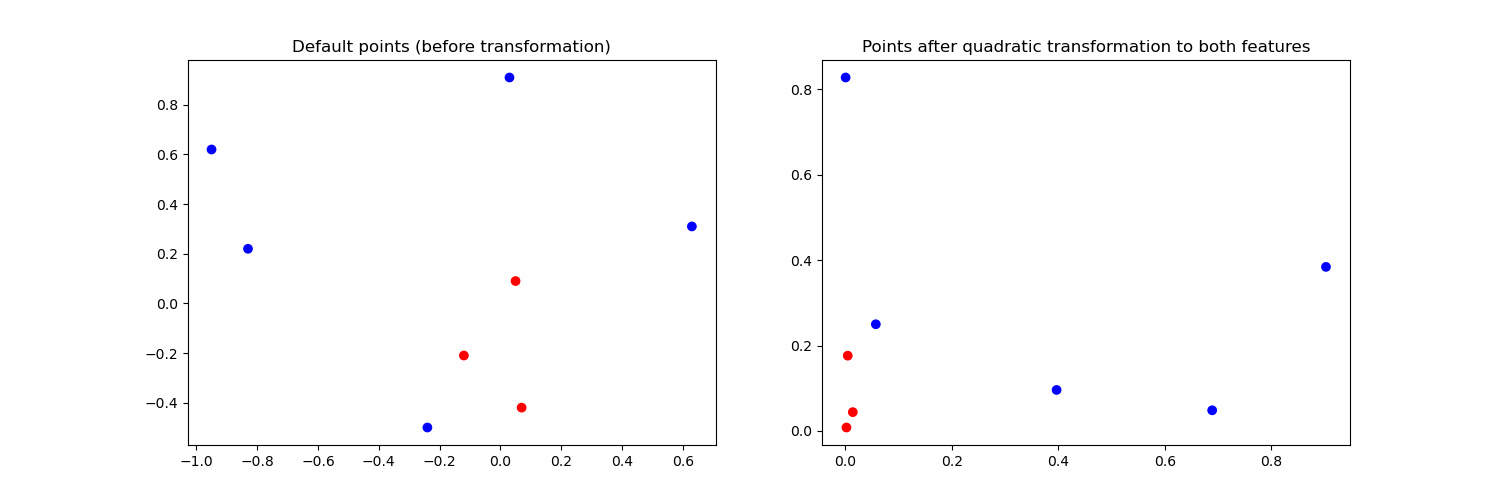
\includegraphics[width=1.1\textwidth]{assets/ex-5/points.png}
        \end{figure}

        In order to sketch the predicted surface, we'll need to find the weight matrix
        associated with the regression; for that, instead of considering the inputs
        matrix, $X$, we're going to consider the transformed inputs matrix, $\Phi$:

        $$
          \Phi(x) = \begin{bmatrix}
            1      & x_1^{(1)} & x_1^{(2)} \\
            \vdots & \vdots    & \vdots    \\
            1      & x_n^{(1)} & x_n^{(2)}
          \end{bmatrix}
        $$

        \begin{align*}
          \Phi = \begin{bmatrix}
  1 & 0.9025 & 0.3844\\
  1 & 0.3969 & 0.0961\\
  1 & 0.0144 & 0.0441\\
  1 & 0.0576 & 0.25\\
  1 & 0.0049 & 0.1764\\
  1 & 0.0009 & 0.8281\\
  1 & 0.0025 & 0.0081\\
  1 & 0.6889 & 0.0484\\
\end{bmatrix}, \quad
          W = (\Phi^T \Phi)^{-1} \Phi^T Z = \begin{bmatrix}
  1.5\\
  -2.22045e-16\\
  -0.5\\
\end{bmatrix}
        \end{align*}

        As such, the regression's equation is given by
        $0.816775 - 0.864807x_1^2 - 0.950784x_2^2$ - \textbf{can't forget that the quadratic
          transformation to the data is not only felt in the weight parameters, but also
          in the input parameters!}.

        \begin{figure}[H]
          \centering
          \includesvg[width=0.7\textwidth]{assets/ex-5/paraboloid.svg}
        \end{figure}

        \question {
  \item Consider both logarithmic and quadratic transformations for the data set below:
  \item
        \begin{table}[H]
          \centering
          \begin{tabular}{c|c|c|c}
                  & $y_1$ & z    \\ \hline
            $x_1$ & 3     & 1.5  \\
            $x_2$ & 4     & 9.3  \\
            $x_3$ & 6     & 23.4 \\
            $x_4$ & 10    & 45.8 \\
            $x_5$ & 12    & 60.1
          \end{tabular}
        \end{table}

        $$
          \phi_1(x_1) = \log(x_1), \quad \phi_2(x_2) = x_2^2
        $$

        \begin{enumerate}
          \item Plot both of the closed form regressions.
          \item Which transformation minimizes the sum of squared errors on the original data?
        \end{enumerate}
        }

        \begin{enumerate}
          \item {
                As it was seen above, using $\Phi$ transformations, we effectively go
                from utilizing the input matrix, $X$, directly, to using the transformed
                input matrix, $\Phi$. For starters, let's compute the transformed input
                matrices, for each transformation:

                $$
                  X = \begin{bmatrix}
  1 & 3 & -1\\
  1 & 4 & 2\\
  1 & 2 & 2\\
\end{bmatrix}, \quad
                  \Phi_1 = \begin{bmatrix}
  1 & 1.09861\\
  1 & 1.38629\\
  1 & 1.79176\\
  1 & 2.30259\\
  1 & 2.48491\\
\end{bmatrix}, \quad
                  \Phi_2 = \begin{bmatrix}
  1 & 9\\
  1 & 16\\
  1 & 36\\
  1 & 100\\
  1 & 144\\
\end{bmatrix}
                $$
                }

                We'll have, then, two weight matrices, $W_1$ and $W_2$, associated with
                each transformation (and, as such, two different linear regressions):

                $$
                  W_1 = (\Phi_1^T \Phi_1)^{-1} \Phi_1^T Z = \begin{bmatrix}
  1.66667\\
  0\\
  -0.333333\\
\end{bmatrix}, \quad
                  W_2 = (\Phi_2^T \Phi_2)^{-1} \Phi_2^T Z = \begin{bmatrix}
  0.77865\\
  0.25955\\
  -0.288854\\
\end{bmatrix}
                $$

                \begin{align*}
                  \hat{z}_1 = -47.0212 + 41.3945 \log(x) \quad
                  \hat{z}_2 = 2.78947 - 0.413615 x^2
                \end{align*}

                \begin{figure}[H]
                  \centering
                  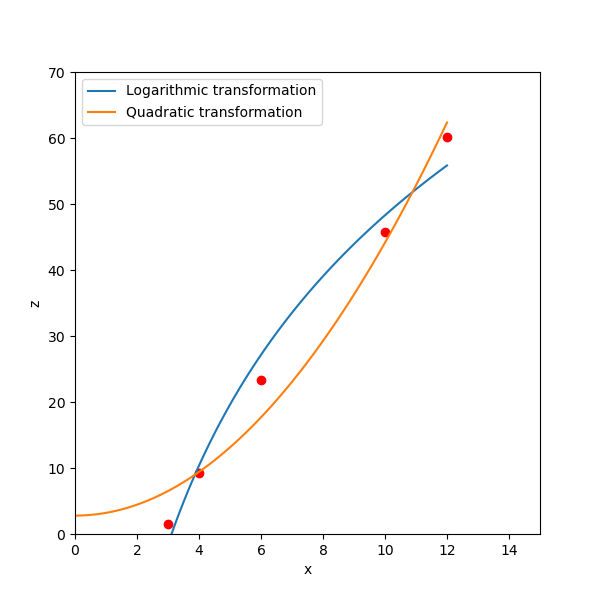
\includegraphics[width=0.35\textwidth]{assets/ex-6/linear-regressions.png}
                \end{figure}
          \item {
                The sum of squared errors for each transformation is rather easy to
                compute:

                \begin{align*}
                  \hat{z}_1 = -47.0212 + 41.3945 \log(x) = \begin{bmatrix}
  -1.54473\\
  10.3637\\
  27.1477\\
  48.2931\\
  55.8402\\
\end{bmatrix}, \quad
                  \hat{z}_2 = 2.78947 - 0.413615 x^2 = \begin{bmatrix}
  6.51201\\
  9.40731\\
  17.6796\\
  44.151\\
  62.3501\\
\end{bmatrix}
                \end{align*}
                \begin{align*}
                  \text{SSE}_1 = \sum_{i=1}^n (z_i - \hat{z}_1)^2 = (1.5 + 1.54473)^2 + \cdots = 48.8088 \\
                  \text{SSE}_2 = \sum_{i=1}^n (z_i - \hat{z}_2)^2 = (1.5 - 6.51201)^2 + \cdots = 65.6365
                \end{align*}
                }

                We choose the model that minimizes the sum of squared errors, which is
                the first one, applying the logarithmic transformation.
        \end{enumerate}

        \question {
  \item Select the criteria promoting a smoother regression model:

        \begin{enumerate}
          \item Applying Ridge and Lasso regularizations to linear regression models.
          \item Increasing the depth of a decision tree regressor.
          \item Increasing the $k$ parameter of a $k$NN regressor.
          \item Parametrizing a $k$NN regressor with uniform weights, instead of the default distance-based weights.
        \end{enumerate}
        }

        In order to answer this question, we need to understand what \textit{smoothing
          a regression model} means. In the context of linear regression, we can say that
        a model is smoother when the weights are smaller - it'll be easier
        to generalize the model to unseen data, avoiding overfitting to training data,
        and to discard noise. In that sense, both LASSO and Ridge regularizations
        are good candidates to smooth a linear regression model.

        Regarding decision trees, smoother models are those with smaller depths -
        very deep trees tend to overfit the data, creating a model whose regression
        is very close to the training data (the regression will shift up and down
        according to the samples it sees in its path). As such,
        increasing the depth of a decision tree regressor will make the model less
        smooth.

        As for $k$NN regressors, it's intuitive that, for both categoric and numeric
        variables, a larger $k$ will make the model smoother - with more samples,
        the mean/mode picked will stabilize, making the model less sensitive to
        noise (and, in the limit case, picking always the same label, regardless
        of the input). As such, we have a smoother model with increasing levels of $k$.

        Finally, regarding the weights of a $k$NN regressor, we can say that the
        utilizing uniform weights leads us to smoother results than the default
        distance-based weights. This is because, with uniform weights, we're
        averaging the labels of the $k$ nearest neighbors, and, as such, the
        model is less sensitive to noise (since the $k$ nearest neighbors will be
        the same for any sample in a certain area of the plane) - if they were distance-based, a single
        coordinate change affects the weights associated of all neighbors, which
        intuitively leads to more variation.
\end{enumerate}

\end{document}